%! Author = Len Washington III
%! Date = 1/17/24

% Preamble
\documentclass[title={Chapter 1}]{fdsn201notes}

% Packages

% Document
\begin{document}

%<*Chapter1>
\maketitle{1}{Nutrition: Linking Food and Health}%

\definecolor{healthpink}{HTML}{ff4c68}
\definecolor{healthgreen}{HTML}{95c82e}
\definecolor{healthblue}{HTML}{1869c3}
\definecolor{healthpurple}{HTML}{c855a5}
\definecolor{healthorange}{HTML}{e97610}

\definecolor{nutrientgreen}{HTML}{3ead44}
\definecolor{nutrientorange}{HTML}{ff9607}
\definecolor{nutrientpink}{HTML}{d8809a}
\definecolor{nutrientred}{HTML}{ff2426}
\definecolor{nutrientpurple}{HTML}{536eb2}
\definecolor{nutrientblue}{HTML}{1581cc}

\section{What is Nutrition?}\label{sec:what-is-nutrition?}

\begin{itemize}
	\item \definition{Nutrition}{the study of food, including}
	\begin{itemize}
		\item How food nourished our bodies
		\item How food influences our health
	\end{itemize}
	\item Nutrition is a relatively new discipline of science.
	\item Nutrition research focuses on supporting health and preventing and/or treating chronic diseases.
	\item Nutrition involves study of the following:
	\begin{itemize}
		\item Food consumption
		\item Food digestion
		\item Food absorption
		\item Food storage
		\item Factors that influence eating patterns
		\item Recommended amounts of types of food
		\item Food safety
		\item The global food supply
	\end{itemize}
\end{itemize}

\section{How Does Nutrition Support Health?}\label{sec:how-does-nutrition-support-health?}
\begin{itemize}
	\item Nutrition supports health and wellness
	\item \definition{Wellness}{A multidimensional, active process by which people make choices to enhance their lives}
	\begin{itemize}
		\item Includes: physical, emotional, social, occupational, and spiritual health
	\end{itemize}
	\item Critical components of wellness
	\begin{itemize}
		\item Nutrition
		\item Physical activity
	\end{itemize}
\end{itemize}

\section{Wellness}\label{sec:wellness}
\textcolor{healthpink}{\subsection{Physical Health}\label{subsec:physical-health}}
Includes nutrition and physical activity.
%
\textcolor{healthgreen}{\subsection{Spiritual Health}\label{subsec:spiritual-health}}
Includes spiritual values and beliefs.
%
\textcolor{healthblue}{\subsection{Emotional Health}\label{subsec:emotional-health}}
Includes positive feelings about one's self and life.
%
\textcolor{healthpurple}{\subsection{Social Health}\label{subsec:social-health}}
Includes family, community, and social environment.
%
\textcolor{healthorange}{\subsection{Occupational Health}\label{subsec:occupational-health}}
Includes meaningful work or vocation.

\section{Nutrition and Chronic Disease Prevention}\label{sec:nutrition-and-chronic-disease-prevention}
\begin{itemize}
	\item Nutrition can prevent disease
	\begin{itemize}
		\item Nutrient-deficiency diseases:
		\begin{itemize}
			\item scurvy (Vitamin-C deficiency)
			\item pellagra
		\end{itemize}
		\item Three chronic diseases strongly associated with poor nutrition:
		\begin{itemize}
			\item Heart disease
			\item Stroke
			\item Diabetes
		\end{itemize}
		\item Diseases in which nutrition plays a role:
		\begin{itemize}
			\item Osteoarthritis
			\item Osteoporosis
		\end{itemize}
	\end{itemize}
	\item Obesity is the primary link between poor nutrition and mortality
\end{itemize}

\begin{figure}[H]
	\centering
	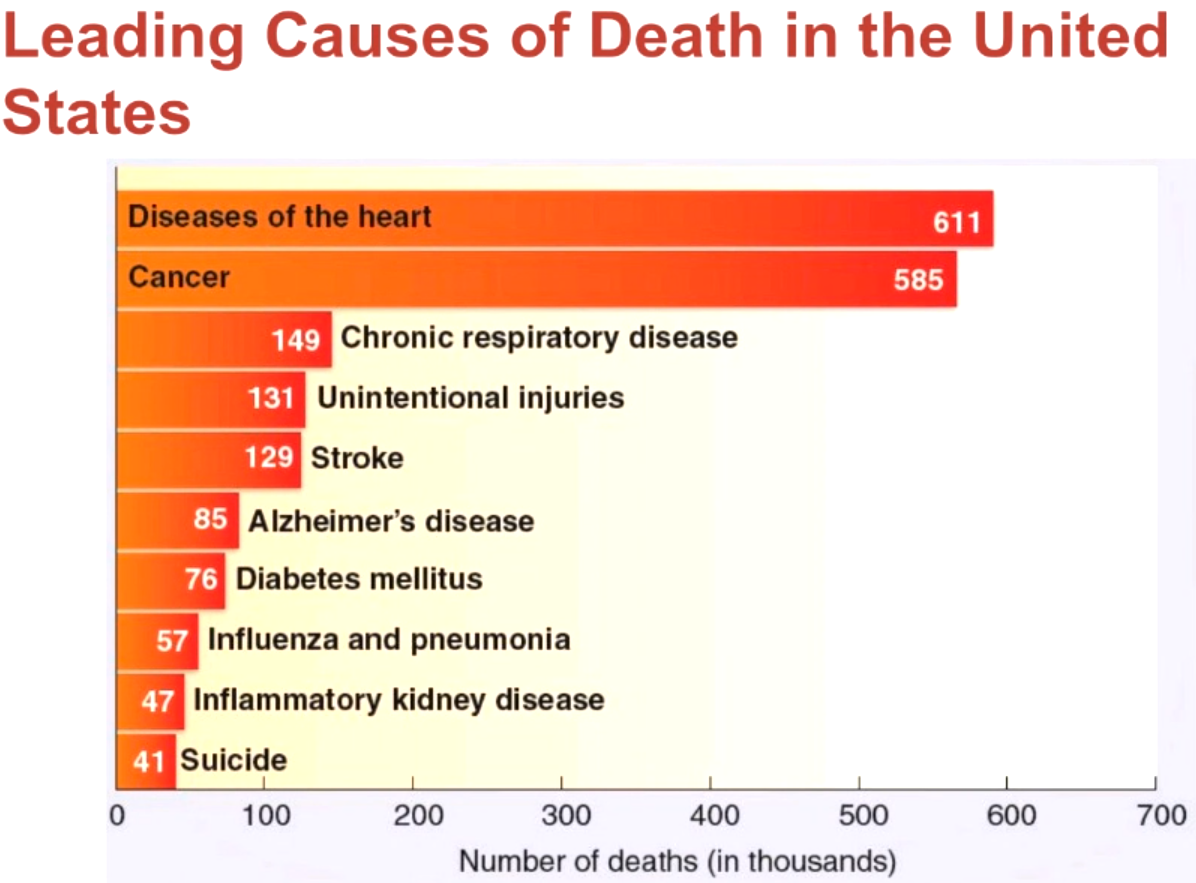
\includegraphics[width=\textwidth]{1_leading_causes_of_death}
	\caption{Leading Causes of Death in the United States}
	\label{fig:leading_causes_of_death_in_us}
\end{figure}

\begin{figure}[H]
	\centering
	\begin{subfigure}[b]{0.475\textwidth}
		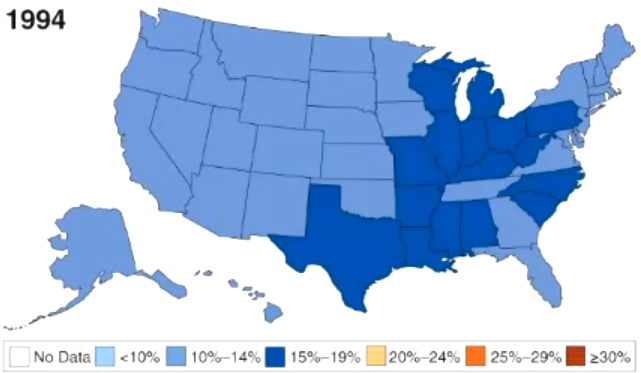
\includegraphics[width=\textwidth]{1_1994_obesity_rates}
		\caption{Obesity rates per U.S. state in 1994.}
		\label{fig:1994_obesity_rates}
	\end{subfigure}
	~
	\begin{subfigure}[b]{0.475\textwidth}
		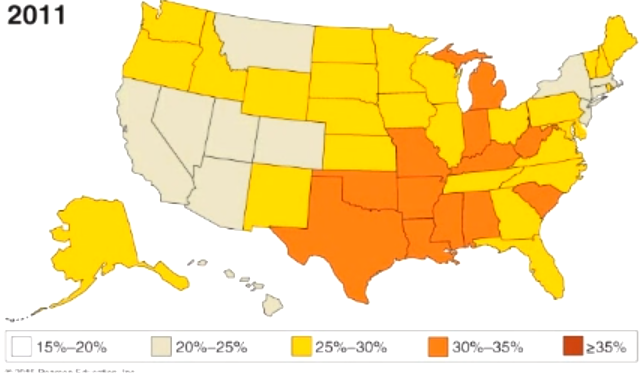
\includegraphics[width=\textwidth]{1_2011_obesity_rates}
		\caption{Obesity rates per U.S. state in 2011.}
		\label{fig:2011_obesity_rates}
	\end{subfigure}
	\caption{A 15-year difference between obesity rates in the United States.}
	\label{fig:15_year_obesity_shift}
\end{figure}

\section{Healthy People 2020}\label{sec:healthy-people-2020}
\begin{itemize}
	\item Nutrition is so important that it has become a national goal
	\item The \emph{Healthy People} plan, revised every decade, identifies goals and objectives to reach by 2020.
\end{itemize}

\subsection{Goals of Healthy People 2020}\label{subsec:goals-of-healthy-people-2020}
\begin{itemize}
	\item Attain high-quality, longer lives free of preventable disease, disability, injury, and premature death
	\item Achieve health equity, eliminate disparities, and improve the health of all groups
	\item Create social and physical environments that promote good health for all
	\item Promote quality of life, healthy development, and healthy behaviors across all life stages
\end{itemize}

\begin{table}[H]
    \centering
    \begin{threeparttable}
		\caption{Weight, Nutrition, and Physical Activity Objecives from \emph{Healthy People 2020}}
		\label{tab:healthy-people-2020}
		\rowcolors{2}{rowmedgreen}{rowlightgreen}
		\begin{tabular}{p{0.35\textwidth} p{0.65\textwidth}}
			\rowcolor{rowdarkgreen}\textbf{Topic} & \textbf{Objective Number and Description}\\
			Weight status & NWS-8. Increase the proportion of adults who are at a healthy weight from 30.8\% to 33.9\%.

			NWS-9. Reduce the proportion of adults who are obese from 34.0\% to 30.6\%.

			NWS-10.2. Reduce the proportion of children aged 6 to 11 years who are considered obese from 17.4\% to 15.7\%.\\
			Food and nutrient composition & NWS-14. Increase the contribution of fruits to the diets of the population aged 2 years and older.

			NWS-15. Increase the variety and contribution of vegetables to the diets of the population aged 2 years and older.\\
			Physical activity & PA--1. Reduce the proportion of adults who engage in no leisure-time physical activity from 36.2\% to 32.6\%.

			PA--2.1. Increase the proportion of adults who engage in aerobic physical activity of at least moderate intensity for at least 150 minutes per week, or 75 minutes per week of vigorous intensity, or an equivalent combination from 43.5\% to 47.9\%.

			PA--2.3. Increase the proportion of adults who perform muscle-strengthening activities on 2 or more days of the week from 21.9\% to 24.1\%.\\
			\rowcolor{rowdarkgreen} & \\
		\end{tabular}
		\begin{tablenotes}
			\small
			\item Data adapted from: \emph{Healthy People 2020 (U.S. Department of Health and Human Services).}
		\end{tablenotes}
	\end{threeparttable}
\end{table}

\section{What Are Nutrients?}\label{sec:what-are-nutrients?}
\begin{itemize}
	\item \definition{Nutrients}{chemicals in foods that are critical to human growth and function}
	\item There are six groups of essential nutrients found in foods:
	\begin{itemize}
		\item \hyperref[subsec:carbohydrates]{Carbohydrates}
		\item \hyperref[subsec:vitamins]{Vitamins}
		\item \hyperref[subsec:fats-and-oils]{Fats and oils}
		\item \hyperref[subsec:minerals]{Minerals}
		\item \hyperref[subsec:proteins]{Proteins}
		\item \hyperref[subsec:water]{Water}
	\end{itemize}
\end{itemize}

\begin{itemize}
	\item \definition{Macronutrients\label{dfn:macronutrients}}{nutrients required in relatively large amounts (grams)}
	\begin{itemize}
		\item Provide energy
		\item Carbohydrates, fats and oils, proteins
	\end{itemize}
	\item \definition{Micronutrients}{nutrients required in smaller amounts}
\end{itemize}

\section{Macronutrients Provide Energy}\label{sec:macronutrients-provide-energy}
\begin{itemize}
	\item We measure energy in kilocalories (kcal)\label{dfn:kcal}
	\item \definition{Kilocalorie}{amount of energy required to raise the temperature of 1 kg of water by 1\textdegree{}C}
	\item On food labels, ``Calorie'' actually refers to kilocalories.
\end{itemize}

\textcolor{nutrientgreen}{\subsection{Carbohydrates}\label{subsec:carbohydrates}}
\begin{itemize}
	\item Provide 4 \hyperref[dfn:kcal]{kcal} per gram.
\end{itemize}
\subsubsection{Functions} Primary energy source of fuel for the body, especially for the brain

\subsubsection{Composed of} Chains of carbon, hydrogen, and oxygen

\subsubsection{Best Sources} Whole grains, vegetables, fruits

\textcolor{nutrientorange}{\subsection{Vitamins}\label{subsec:vitamins}}
\subsubsection{Functions} Important source of energy at rest during low-intensity exercise

\subsubsection{Composed of} Carbon, hydrogen, and oxygen

\subsubsection{Best Sources} Vegetable oils, butter and dairy products

\textcolor{nutrientpink}{\subsection{Fats and oils}\label{subsec:fats-and-oils}}
\begin{itemize}
	\item Fats are composed of \hyperref[dfn:lipids]{lipids}, molecules that are insoluble in water
	\item Provide 9 \hyperref[dfn:kcal]{kcal} per gram.
	\item Fats are an important source of fuel for our bodies during times of rest or low-intensity exercise
	\item Our bodies can store fat which can be used for energy while we are not eating
	\item Source of fat-soluble vitamins and essential fatty acids
\end{itemize}
\subsubsection{Functions} Support tissue growth, repair and maintenance

\subsubsection{Composed of} Amino acids made up of carbon, hydrogen, oxygen and nitrogen

\subsubsection{Best Sources} Meats, dairy products, seeds, nuts, legumes

\textcolor{nutrientred}{\subsection{Minerals}\label{subsec:minerals}}
\subsubsection{Functions} Assist with release of macronutrients; critical to building and maintaining bone, muscle, and blood; support immune function and vision

\subsubsection{Composed of} fat-soluble and water-soluble compounds

\subsubsection{Best Sources} fruits, vegetables, dairy products, meats

\textcolor{nutrientpurple}{\subsection{Proteins}\label{subsec:proteins}}
\begin{itemize}
	\item Proteins are chains of amino acids
	\item Can supply 4 kcal of energy per gram, but are not usually a primary energy source
	\item Important for:
	\begin{itemize}
		\item Building cells and tissues
	\end{itemize}
\end{itemize}
\subsubsection{Functions} Assist with fluid regulation and energy production; maintain health of blood and bones; rid body of harmful by-products of metabolism

\subsubsection{Composed of} Carbon,  %Single elements such as sodium, potassium, calcium or iron

\subsubsection{Best Sources} Fruits, vegetables, dairy products, meats

\textcolor{nutrientblue}{\subsection{Water}\label{subsec:water}}
\subsubsection{Functions} Ensures proper fluid balance; assists in regulation of nerve impulses, body temperature, and muscle contractions

\subsubsection{Composed of} Hydrogen and oxygen

\subsubsection{Best Sources} Water, juices, soups, fruits, vegetables
% Stopped at 25:29

\section{Micronutrients}\label{sec:micronutrients}
\begin{itemize}
	\item Vitamins and minerals (and \hyperref[dfn:phytochemicals]{phytochemicals}/phytonutrients) are known as micronutrients
	\item \definition{Micronutrients}{Nutrients needed in relatively small amounts to support normal health and body functions}
	\item Neither vitamins not minerals provide kilocalories
\end{itemize}

\subsection{Vitamins}\label{subsec:vitamins-2}
\begin{itemize}
	\item \definition{Vitamins}{organic molecules that assist in regulating body processes}
	\item Vitamins are classified by the way they are absorbed, transported, and stored in the body
	\begin{itemize}
		\item Fat-soluble vitamins
		\item Water-soluble vitamins
	\end{itemize}
\end{itemize}

\begin{table}[H]
	\centering
	\caption{Overview of Vitamins}
	\label{tab:vitamin-overview}
	\rowcolors{2}{rowmedgreen}{rowlightgreen}
	\begin{tabular}{p{0.1\textwidth} p{0.3\textwidth} p{0.6\textwidth}}
		\rowcolor{rowdarkgreen}\textbf{Type} & \textbf{Names} & \textbf{Distinguishing Features}\\
		Fat soluble & A, D, E, K & Soluble in fat

		Stored in the human body

		Toxicity can occur from consuming excess amounts, which accumulate in the body\\
		Water soluble & C, B-vitamins (thiamin, riboflavin, niacin, vitamin $\mbox{B}_{6}$, vitamin $\mbox{B}_{12}$, pantothenic acid, biotin, folate) & Soluble in water

		Note stored to any extent in the human body

		Excess excreted in urine

		Toxicity generally only occurs as a result of vitamin supplementation\\
		\rowcolor{rowdarkgreen} & & \\
	\end{tabular}
\end{table}

\subsection{Minerals}\label{subsec:minerals-2}
\begin{itemize}
	\item \definition{Minerals}{inorganic (cannot be broken down) substances required for body processes}
	\begin{itemize}
		\item Minerals include sodium, calcium, iron, potassium, and magnesium
		\item Minerals have many different functions, such as fluid regulation and energy production; are essential to bones and blood; and help eliminate harmful by-products of metabolism
	\end{itemize}
\end{itemize}

\begin{table}[H]
	\centering
	\caption{Overview of Minerals}
	\label{tab:mineral-overview}
	\rowcolors{2}{rowmedgreen}{rowlightgreen}
	\begin{tabular}{p{0.1\textwidth} p{0.3\textwidth} p{0.6\textwidth}}
		\rowcolor{rowdarkgreen}\textbf{Type} & \textbf{Names} & \textbf{Distinguishing Features}\\
		Major Minerals & Calcium, phosphorus, sodium, potassium, chloride, magnesium, sulfur & Needed in amounts greater than 100 mg/day in our diet

		Amount present in the human body is greater than 5 g (5,000 mg)\\
		Trace minerals & Iron, zinc, copper, manganese, fluoride, chromium, molybdenum, selenium, iodine & Needed in amounts less than 100 mg/day in our diet

		Amount present in the human body is less than 5 g (5,000 mg)\\
		\rowcolor{rowdarkgreen} & & \\
	\end{tabular}
\end{table}

\subsection{Water Supports All Body Functions}\label{subsec:water-supports-all-body-functions}
\begin{itemize}
	\item Water is an inorganic nutrient that is vital for health and survival
	\item Water is involved in many bodily processes:
	\begin{itemize}
		\item fluid balance
		\item nutrient transport
		\item nerve impulses
		\item removal of wastes
		\item muscle contractions
		\item body temperature
	\end{itemize}
\end{itemize}

\section{Determining Nutrient Needs}\label{sec:determining-nutrient-needs}
\begin{itemize}
	\item Dietary Reference Intakes (DRIs) identify the
	\begin{itemize}
		\item Amount of a nutrient needed to prevent deficiency disease in healthy people
		\item Amount of a nutrient that may reduce the risk of chronic disease
		\item Upper level of safety for nutrient intake
	\end{itemize}
	\item DRIs consist of four values
	\begin{itemize}
		\item Estimated Average Requirement (EAR)
		\item Recommended Dietary Allowance (RDA)
		\item Adequate Intake (AI)
		\item Tolerable Upper Intake Level (UL)
	\end{itemize}
\end{itemize}

\subsection{Estimated Average Requirement (EAR)}\label{subsec:estimated-average-requirement-(ear)}
\begin{itemize}
	\item The average daily intake level of a nutrient that will meet the needs of half of the healthy people in a particular life stage and gender group
	\item Used to determine the Recommended Dietary Allowance (RDA) of a nutrient
\end{itemize}

\subsection{Recommended Dietary Allowance (RDA)}\label{subsec:recommended-dietary-allowance-(rda)}
\begin{itemize}
	\item The average daily intake level required to meet the needs of 97--98\% of health people in a particular life stage and gender group
\end{itemize}

\subsection{Adequate Intake (AI)}\label{subsec:adequate-intake-(ai)}
\begin{itemize}
	\item Recommended average daily intake level for a nutrient that is assumed to be adequate
	\item Based on observations and estimates from experiments
	\item Used when the RDA is not yet established: vitamin D, vitamin K, fluoride, and chromium
\end{itemize}

\subsection{Tolerable Upper Intake Level (UL)}\label{subsec:tolerable-upper-intake-level-(ul)}
\begin{itemize}
	\item Highest average daily intake level that is not likely to have adverse effects on the health of most people
	\item Consumption of a nutrient at levels above the UL is not considered safe
\end{itemize}

\section{DRIs and Energy}\label{sec:dris-and-energy}
\begin{itemize}
	\item Two DRIs apply to energy specifically
	\begin{itemize}
		\item Estimated Energy Requirement (EER)
		\item Acceptable Macronutrient Distribution Range
	\end{itemize}
\end{itemize}

\subsection{Estimated Energy Requirement (EER)}\label{subsec:estimated-energy-requirement-(eer)}
\begin{itemize}
	\item Average dietary energy intake to maintain energy balance
	\item Based on age, gender, weight, height, and level of physical activity
\end{itemize}

\subsection{Acceptable Macronutrient Distribution Range (AMDR)}\label{subsec:amdr}
\begin{itemize}
	\item The range of energy intake from carbohydrate, fat and protein associated with reduced risk of chronic disease
	\item The range of macronutrient intake that provides adequate levels of essential nutrients
\end{itemize}

\section{Interpreting Nutrition Research}\label{sec:interpreting-nutrition-research}
\begin{itemize}
	\item Research involves applying the scientific method
	\begin{itemize}
		\item Observation and description of a phenomenon
		\item Creation of a hypothesis
		\item Design of a repeatable experiment
		\item Collection, analysis, and interpretation of data
		\begin{itemize}
			\item Formation of a conclusion, or proposal of an alternative hypothesis
		\end{itemize}
		\item Development of a theory based on repeated experiments
	\end{itemize}
\end{itemize}

\section{Types of Research Studies}\label{sec:types-of-research-studies}
\begin{itemize}
	\item Animal versus human studies
	\begin{itemize}
		\item Drawbacks: ethical concerns, and results may not apply to humans
	\end{itemize}
	\item Epidemiological studies
	\item Observational studies
	\begin{itemize}
		\item Can only indicate relationships between factors
	\end{itemize}
	\item Case control studies
	\item Clinical trials
\end{itemize}

\subsection{Clinical Trials}\label{subsec:clinical-trials}
\begin{itemize}
	\item In clinical trials, an intervention's effect on a certain disease or health condition is tested using two groups: the experimental group and the control group
	\item Randomized trials
	\item Single- and double-blind experiments
	\begin{itemize}
		\item Placebo: an imitation treatment that has no effect, given to the control group in placebo-controlled double-blind randomized clinical trials
	\end{itemize}
\end{itemize}

\section{Evaluating Nutrition-Related Claims}\label{sec:evaluating-nutrition-related-claims}
\begin{itemize}
	\item Ask these questions to determine scientific validity:
	\begin{itemize}
		\item Who is reporting the information?
		\begin{itemize}
			\item What are their credentials?
		\end{itemize}
		\item Who conducted the research and who paid for it?
		\begin{itemize}
			\item Is there a conflict of interest?
		\end{itemize}
	\end{itemize}
	\item Is the report based on reputable research studies?
	\begin{itemize}
		\item Was there a control and an experimental group?
		\item Was the sample size large enough to rule out chance variation?
		\item Was a placebo effectively administered?
		\item Was it a double-blind study?
	\end{itemize}
	\item Is the report based on testimonials?
	\item Are the claims too good to be true?
\end{itemize}

\section{Determining a Website's Reliability}\label{sec:determining-a-website's-reliability}
Look at:
\begin{itemize}
	\item The website sponsors' credentials
	\item Whether the date of the website is recent
	\item The Internet address: ``.gov'', ``.edu'' and ``.org'' are generally considered reliable
\end{itemize}

\section{Whom Can You Trust?}\label{sec:whom-can-you-trust?}
\begin{itemize}
	\item Trustworthy experts are educated and credentialed
	\begin{itemize}
		\item Registered dietitian (RD)
		\item Licensed dietitian
		\item Nutritionist with credentials and experience
		\item Professional with advanced degree(s) in nutrition (MS, MA, or PhD in nutrition)
		\item Physician with appropriate expertise in nutrition
	\end{itemize}
	\item Government agencies are usually trustworthy
	\begin{itemize}
		\item The Centers for Disease Control and Prevention (CDC) supports two large national surveys
		\begin{itemize}
			\item National Health and Nutrition Examination Survey (NHANES)
			\item Behavioral Risk Factor Surveillance System Survey (BRFSS)
		\end{itemize}
	\end{itemize}
	\item National Institutes of Health (NIH) focuses on specific areas of research, including cancer; heart, lung, and blood diseases; diabetes; and alternative medicine
	\item Professional organizations publish cutting-edge nutrition research and information
	\item These include
	\begin{itemize}
		\item Academy of Nutrition and Dietetics (AND)
		\item American Society for Nutrition (ASN)
		\item American College of Sports Medicine (ACSM)
		\item The Obesity Society (TOS)
	\end{itemize}
\end{itemize}

\section{In Depth: New Frontiers}\label{sec:in-depth:-new-frontiers}
\begin{itemize}
	\item \definition{Nutrigenomics}{studies the interactions among genes, the environment, and nutrition}
	\begin{itemize}
		\item Key theory: foods and environmental factors can ``switch'' some genes on while turning off others
		\item Could help in reducing risk of diet-related disease, treating existing conditions through diet, and making personalized nutrition possible
	\end{itemize}
	\item The human genome is the set of genes making up the DNA in the nucleus of a human cell
	\item The human microbiome is the set of genes belonging to microorganisms that inhabit the human body
	\begin{itemize}
		\item Our health is affected by the way they interact with our human cells and genes that are required for digestion
		\item GI flora: helpful bacteria in our gastrointestinal (GI) tract
	\end{itemize}
	\item Functional foods have biologically active ingredients that provide health benefits beyond basic nutrition
	\begin{itemize}
		\item \definition{Probiotics}{contain live microorganisms that improve the intestinal microbial balance}
		\item \definition{Prebiotics}{nondigestible food ingredients that stimulate the growth and/or activity of probiotic bacteria}
		\item \definition{Phytochemicals\label{dfn:phytochemicals}}{naturally occuring plant compounds believed to have health-promoting effects in humans}
	\end{itemize}
\end{itemize}

%</Chapter1>

\end{document}